%KELOMPOK 4 Blank-On1
%\begin{enumerate}
%\item Andri Fajar Sunandhar
%\item Cokro Edi Prawiro
%\item Fadila
%\item Sandro Samuel Sinaga
%\end{enumerate}



\section{Common Gateway Interface}
CGI merupakan metode yang dipakai untuk mempertukarkan data di antara server dan klien (browser). CGI merupakan sebuah standar dimana program atau script bisa mengirim data kembali ke web server dimana ia diproses, yaitu dengan menggunakan tag HTML standar untuk mendapatkan data dari seseorang, kemudian meneruskannya ke CGI. Selanjutnya CGI melakukan serangkaian aksi terkait data tersebut\cite{prihatmoko2013pengembangan}.



\par CGI adalah interface untuk menjalankan program-program eksternal,dibawah informasi server, biasanya server HTTP (walaupun CGI standar dirancang untuk lintasan-platform yang
menangani semua jenis hardware dan software yang berbeda, windows CGI 1.3 khusus untuk platform microsoft Windows 95/98 dan windows NT). Dengan CGI server bisa
melayani informasi yang tidak ada dalam format yang mudah dibaca oleh client,seperti data yang ada dalam database SQL, dan melakukan gateway antara dua sesuatu yang 
dihasilkan oleh browser client. Seringkali program gateway ini disebut script.

\par Sebuah server web memproses permintaan klien CGI menggunakan skrip atau aplikasi CGI. Sebagai contoh, ketika sebuah database ditanyakan oleh klien, 
server web bertindak sebagai gateway antara database dan klien. Server web mentransmisikan permintaan klien ke aplikasi CGI yang melakukan kueri basis data,
 memformat hasil dan mengembalikan data berformat HTML ke server web. Server web kemudian mentransmisikan data berformat HTML ke klien untuk ditampilkan kepada pengguna.

\par Di server, protokol yang diperluas lebih didukung oleh antarmuka gerbang umum (CGI) yang mengubah komunikasi dari perangkat I / O non-standar ke format yang kompatibel 
dengan transaksi atau program aplikasi data yang dapat dijalankan pada server atau komputer yang dipasangkan ke server. 
Dengan cara ini, CGI memungkinkan pemrosesan perintah kemampuan yang diperluas untuk dipisahkan dari fungsi komunikasi yang dilakukan oleh server.

\par Adapun pengertian lain dari Common Gateway Interface yaitu sekumpulan aturan untuk mengarahkan sebuah server web berkomunikasi dengan software dalam mesin yang sama begitu pula sebaliknya antara software CGI programs dengan web server. Setiap perangkat lunak dapat menjadi perogram CGI dengan syarat software tersebut dapat melakukan input dan output sesuai setandar CGI. CGI menjadi setandar menghubungkan untuk menghubungkan data informasi yang terjadi antara server dan aplikasi, seperti HTTP. Script CGI dapat mengirtimkan data kembali ke web server  dimana CGI diperoses. CGI merupakan interface antara halaman website dengan web server yang menjalankan perogram\cite{aditya2015analisis}.

\begin{figure}[ht]
\centerline{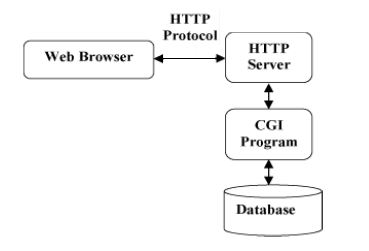
\includegraphics[width=1\textwidth]{figures/2arsitekturCGI.JPG}}

\caption{CGI Arsitektur Diagram} 
\label{2arsitekturCGI}
\end{figure}

Gambar\ref{2arsitekturCGI} menjelaskan bahwa antara HTTP server di pelantarai oleh CGI program dalam mengakses data 
dari database. Jadi jika data yang diminta di batasi atau tidak memiliki hak akses oleh CGI data tersebut tidak dapat di munculkan 
oleh web browser.  Cara untuk memahami perinsip dari (Common Gateway Interface ) CGI, dapat dicoba dengan melakukan click pada suatu URL suatu website.
setelah melakukan hal tersebut browser akan menghubungi HTTP web server dan meminta URL dari website tersebut. Kemudian web server tersebut akan
mengurai (prasing) URL dan akan mencari berkas dari link tersebut, bila ditemukan maka akan diteruskan ke browse, begitu juga sebaliknya jika tidak ada
maka akan diberikan pesan error. lalu web browser akan menampilkan hasilnya, baik url yang tadi diminta maupun pesan error karena URL yang dituju tidak ada. Meski begitu, ada kemungkinan untuk mengatur suatu HTTP server untuk membatasi akses terhadap suatu berkas.
jadi halaman URL yang dituju tidak bisa diakses hal tersebut merupakan fungsi dari CGI script. supaya lebih paham dapat dilihat 
pada arsitektir program CGI.

\par  CGI (Common Gateway Interface) memungkinkan server web memanggil suatu program, lalu mengirimkan data-data spesifik dari pengguna ke program tersebut.
 Hasil proses tadi diterima oleh CGI yang selanjutnya menyerahkannya kepada server web untuk kemudian, yang pada gilirannya akan mengirimkan
informasi tersebut kembali dalam bentuk HTML ke browser web pengguna, Server web kemudian mentransmisikan data berformat HTML ke klien untuk ditampilkan kepada pengguna. \cite{ibrahim2011sistem}.

\section{PHP and Common Gateway Interface interconnections }
\textit {Common Gateway Interface is a standard that is used to connect various application programs to web pages. One example of the programming language is PHP. PHP is a software that is open source and can pass across the various platform. Php can be run in 2 ways ie as apache module in web server and also as binary in Common Gateway Interface.This language was created in 1994 by Ramus Lerdoff.  Initially, PHP is a CGI program that is devoted to receiving input through forms displayed in web pages or browser. The PHP code is usually processed by a PHP interpreter which is usually executed as a native web server module or Common Gateway Interface}\cite{nahado2015bumbu}.


\section{Security in Common Gateway Interface }
\textit {Common Gateway Interface is used to connect WWW (World Wide Web) systems with software or other software on the web server. The presence of the Common Gateway Interface allows connection interactive between the user and also the web server. Common Gateway Interface itself is often used as a mechanism to get information from users through "fill out a form", access the database, or generate dynamic pages. Although in principle the mechanisms in the Common Gateway Interface do not have security holes, programs or scripts created as CGI can have security flaws either created intentionally or unintentionally. That is because CGI program itself is run on the web server to use the web server resources}\cite{afrianto2015materi}.


\section{The Application of Common Gateway Interface }
\textit {CGI is applied to the making of applications involving python language with PHP language. CGI itself is implemented or modified as CGI Fast CGI protocol, where its function in the application is as an interface in other applications to the web server which is an alternative facility to improve its own performance for CGI which is intended for the web server application process which is Apache web server to dynamic language another. Processes and handling from CGI to FastCGI can be demonstrated from the use of this working support facility such as python as the dynamic language used and the fastCGI module for the server to be used on RFC2109 proxy caching}\cite{kridoyono2017optimasi}.


\section{ Web Database and Common Gateway Interface Interconnections }
\textit {The Internet database development platform is adapted for approaches by connecting with or from CGI (Common Gateway Interface). The technical description includes a discussion of the Common Gateway Interface in which CGI functions as an interface for executing information on external programs, under server information, usually HTTP servers (although the Common Gateway Interface standard is designed for path-platforms that handle all different hardware and software.) Using a CGI server can serve information that does not exist in a format that is easy to read by the client, such as in existing data in SQL databases, and performs a gateway between two things generated by the client browser, which is usually the gateway program called scripts}.


\section{Honeypot}
Menurut Lance Spitzner Honeypot adalah sumber daya keamanan yang mempunyai nilai jika sistem disusupi atau diserang. Pada dasarnya Honeypot merupakan suatu alat untuk mendapatkan informasi dari penyerang. Honeypot merupakan sistem yang dirancang untuk diperiksa dan diserang.
Honeypot Dionaea merupakan salah satu Honeypot interaksi rendah yang bertujuan menangkap salinan malware berbahaya yang masuk ke dalam sistem. Malware tersebut biasanya ada pada layanan yang ditawarkan dalam jaringan. Dionaea menggunakan Python sebagai bahasa script dan libemu sebagai pemecah kode. Dionaea mendukung Internet Protocol v6 dan Transport Layer Security (TLS)\cite{andros2015implementasi}.

\section{Web Server Gateway Interface (WSGI) }
Salah satu keunggulan yang dijelaskan sebelumnya adalah karena Google App Engine dan Django dirancang untuk menggunakan standar WSGI untuk menjalankan aplikasi.
Django dapat berjalan dengan lingkungan server yang berbeda. Misalnya yang populer Server Apache didukung menggunakan mod python atau mod wsgi.
Juga untuk python maprelational Objectperational mendukung PostgreSQL, MySQL, SQLite dan Oracle.

\par Sebuah server web diatur di atas sistem operasi untuk mengirim permintaan HTTP, tetapi juga bisa melayani file statis seperti gambar, file JavaScript, halaman HTML, dll.
 Itu memproses pesan JSON dengan Flask, yang merupakan kerangka mikro untuk Python yang difokuskan pada kode aplikasi web, Karena server web tidak dapat berkomunikasi
 secara langsung dengan Flask, kami mengimplementasikan Web Server Gateway Interface (WSGI) untuk bertindak sebagai proxy antara server dan Python / Flask.

\section{ Python Program Langguage and Common Gateway Interface Interconnections }
\textit {In an application development with python programming language can be seen the relationship between Common Gateway Interface with python itself. Python programming language that is intepreter so that supports access in realtime (right at the point) in the data retrieval or the results of monitoring data. Another reason that is taken and considered is because the Python programming language using the OOP approach of Object Oriented Pprogramming so ideal and suitable for dingunakan on web programming in the Common Gateway Interface (CGI). To run the monitoring system as in the application to be built is very possible once to use or utilize the program interface that can bridge and help users through the web browser on the remote terminal. The interface of this program is called CGI or Common Gateway Interface which can usually be found by users and available on linux}\cite{ohara2005aplikasi}.

\section{Penyokong Aplikasi Web berbasis Python}
\par Perlu anda ketahui bahwa web berbasis Python memiliki beberapa penyokong untuk membuat website yangbaik.
Sebelum mengetahui apa saja penyokong webbsite Python alangkah lebih baiknya mengetahui apa Python itu.
Python adalah bahasa pemerograman yang dinamik, yang banyak digunakan secara luas dari banyak domain aplikasi, 
seperti pengembangan website dan internet, akses basisdat, Dekstop Graphical User Interface, ilmiah dan numerik, pendidikan,
pemerograman jaringan, permainan, dan Grapik 3D. dapat berjalan pada semua sistem oprasi, seperti linux, Windows, Mac, dan lainnnya.
bahasa pemerograman ini memiliki lisensi open-source yang dapat dengan gratis digunakan atau didistribusikan bahkan untuk penggunaan komersial\cite{andros2015implementasi}.

\subsection{Supervisord}
\par Perlu diketahui bahwa sebuah website memiliki tenggang waktu untuk tetap hidup, slah satu fungsi dari Supervisord adalah untuk mengaktifkan 
kembali sebuah website. Jika terjadi banyak permintaan (request) dan web server mati, maka untuk mengaktifkannya kembali harus masuk masuk ke server secara manual.
Dengan menggunakan supervisord hal trsebut dapat ditangani. Selain itu Supervisord merupakan alat untuk memonitoring sejumlah proses yang ada di bawahnya.  

\subsection{Gunicorn}
\par Green Unicorn yang kemudian disingkat menjadi `Gunicorn'merupakan sebuah HTTP Server yang digunakan untuk python, berbasis webserver gateway interface `WSGI' dan dikhususkan 
untuk lingkungan Unix-Like. Sebenarnya Gunicorn merupakan proyek yang diambil dari proyek Unicron untuk Ruby. Gunicorn memiliki penyesuaian yang sangat tinggi terhadap web berbasis WSGI 
seperti Django, Falcon dan lainnya. adapun beberapa fitur unggul dari Gunicorn antara lain :


\begin{enumerate}
\item Dukungan terhadap WSGI, Django, dan Paster
\item Manajemen prose worker secaraotomatis
\item Konfigurasi yang mudah
\item Konfigurasi pada banyak worker
\item Berbagai macam server hooks untuk extensibilitas
\item Kopatibel dengan Python 2.x atau 3.x
\end{enumerate}
